% !TeX spellcheck = en_US
\chapter{Probabilities}
\label{cha:probabilities}

\section{Definitions}
\label{sec:prob-defs}

\subsection{Basic Definitions}
\begin{itemize}
	\item If $x$ is discrete: $\underset{x}{\sum} p(x) = 1$ with $\forall$ $0 \leq p(x) \leq 1$
	\item If $x$ is continuous: $\displaystyle \int p(x) \,dx = 1 \Rightarrow \exists$ a \textbf{\ac{pdf}}\\
	$p(x)$ can take any positive value, as long as \(\displaystyle \int p(x) \,dx = 1\)\\
	\todo{Add image}\\
	\note: theoretically $p(x) = 0, \forall x$
	\item Common types
	\begin{align*}
		& \text{Joint probability:} 		&& p(x_i, y_i) 	&& \left(= p(X=x_i, Y=y_i)\right) \\
		& \text{Marginal probability:} 		&& p(x_i) 		&& \left(= p(X=x_i)\right) \\
		& \text{Conditional probability:} 	&& p(y_i | x_i) && \left(= p(Y=y_i|X=x_i)\right)
	\end{align*}	
	\item Sum rule: $\displaystyle \sum$ joint \ac{prob} = marginal \ac{prob}\\
	$\Rightarrow$ Marginalization	
	\begin{itemize}
		\item discrete variable: $\displaystyle p(x)=\underset{y}{\sum} p(x, y)$
		\item continuous variable: $\displaystyle p(x) = \int p(x,y) dy$
	\end{itemize}
	\item Product rule: Product of marginal \ac{prob} and conditional \ac{prob} = joint \ac{prob}
\end{itemize}

\subsection{Independence and Variability}
\begin{itemize}
	\item Independence. \Eg: $x, y$ are independent, then
	\[\begin{cases}
		p(x|y) = p(x)\\
		p(y|x) = p(y)
	\end{cases}
	\iff p(x,y) = p(x).p(y)\]
	
	\item Variability
	\begin{itemize}
		\item variance:\\ $var \left[f\right] = \expectation{\left(f(x)-\expectation{f(x)}\right)^2} = \expectation{f(x)^2} - \expectation{f(x)}^2$
		\item covariance:\\ $cov \left[x, y\right] = \mathbb{E}_{x,y}\left[xy\right] - \expectation{x}.\expectation{y} = \mathbb{E}_{x,y}\left[xy^T\right] - \expectation{x}.\expectation{y^T}$
		\item covariance matrix
	\end{itemize}
\end{itemize}

\subsection{Bayes Rule}
\label{subsec:bayes-rule}
\begin{align*}
	& p(x_i|y_i).p(y_i) = p(y_i|x_i).p(x_i) = p(x_i, y_i) \\
	\Rightarrow\; &p(y_i|x_i) = \frac{p(x_i|y_i).p(y_i)}{p(x_i)} = \frac{p(x_i|y_i).p(y_i)}{\underset{y}{\sum} p(x_i|y_i).p(y_i)}
\end{align*}
$\Rightarrow$ the \hlb{Bayes equation}:\\~\\
\hlre{posterior = \frac{likelihood \times prior}{normalization~factor}}

\subsection{Expectation}
\label{subsec:expectation}
\begin{align*}
	& \text{For variable $x$:} && \expectation{x} = \underset{x}{\sum}x.p(x) && \left( = \int x.p(x)dx \right)\\
	& \text{For function $f(.)$:} && \expectation{f(x)} = \underset{x}{\sum}f(x).p(x) && \left( = \int f(x).p(x)dx \right)
\end{align*}

\section{Types of Probability Distributions}
Reference source: \href{https://machinelearningcoban.com/2017/07/09/prob/}{machinelearningcoban.com}.
\subsection{Bernoulli Distribution}
Bernoulli Distribution is a distribution to describe binary discrete variables. It's the case that the variable can only take value in 2 classes $x \in \{0,1\}$. \Eg, the probability of throwing a coin. The Bernoulli distribution is defined with parameter $\lambda \in[0,1]$:
\begin{equation}
	p(x) = \text{Bern}_x[\lambda] = \begin{cases}
		p(x=1) = \lambda\\
		p(x=0) = 1-\lambda
	\end{cases}
\end{equation}
In short form, the above equation can be combined into one:
\begin{equation}
	p(x) = \lambda^x(1-\lambda)^{(1-x)} \Rightarrow
	\begin{cases}
		p(0) = \lambda^0 (1-\lambda)^1 = 1-\lambda \\
		p(1) = \lambda^1 (1-\lambda)^0 = \lambda \\
	\end{cases}
\end{equation}

\subsection{Categorical Distribution}
\label{subsec:categorical-distribution}
\textit{Categorical Distribution} is the generalization of \textit{Bernoulli Distribution}, in case there are $K$ classes for the discrete variable $x \in \{ 1, 2, \dots, K\}$. Accordingly, there will be $K$ parameters to describe this \ac{pdf}: $\lambda = [\lambda_1, \lambda_2, \dots, \lambda_K]$, with $\lambda_k \geq 0$ and $\sum \lambda_k = 1$. Each $\lambda_k$ represents the probability to take the output $k$: $p(x = k) = \lambda_k$. In short: $p(x) = \text{Cat}_x [\lambda]$.

Another common way to represent the output is the one-hot vector, $\mathbf{x} \in \{\mathbf{e}_1, \mathbf{e}_2, \dots, \mathbf{e}_K\}$ with $\mathbf{e}_k$ is the $k$-unit vector, which has all 0-element, except the $k$-element equal to 1. \Eg, given 3 classes: $\textbf{e}_1 = [1, 0, 0]^T, \textbf{e}_2 = [0, 1, 0]^T, \textbf{e}_3 = [0, 0, 1]^T$. We will then have:
\begin{equation}
	p(\mathbf{x} = \mathbf{e}_k) = \prod_{j=1}^K \lambda_j^{x_j} = \lambda_k
\end{equation}
because for $\textbf{x}=\textbf{e}_k$, only $x_k=1$, while $x_j = 0, \forall j\neq k$.

\subsection{Univariate Normal Distribution}
Univariate Normal Distribution is also known as the Gaussian distribution. For single dimension data (in 1D): $x \in (-\infty, \infty)$, the mean $\mu \in \mathbb{R}$, and the variance $\sigma^2$ with $\sigma \in \mathbb{R}$.
\begin{equation}
	p(x) = \text{Norm}_x\left[\mu, \sigma^2\right] = \mathcal{N}(\mu, \sigma^2) = \frac{1}{\sqrt{2\pi\sigma^2}}.\text{exp}\left(-\frac{(x-\mu)^2}{2\sigma^2}\right)
\end{equation}
\note
\begin{itemize}
	\item \hlr{Marginals \ac{prob} of Gaussian are again Gaussian.}
	\item When estimating the \ac{param} of a Gaussian, beware the underestimation problem.
	\begin{align*}
		\expectation{\mu_{ML}} &= \mu \\
		\expectation{\sigma^2_{ML}} &= \left(\frac{N-1}{N}\right)\sigma^2 \\
		\Rightarrow \overset{\sim}{\sigma}^2 &= \left(\frac{N}{N-1}\right)\sigma^2_{ML} = \frac{1}{N-1} \sum_{n=1}^{N} (x_n-\hat{\mu})^2
	\end{align*}
\end{itemize}
\begin{figure}[hbt!]
	\centering
	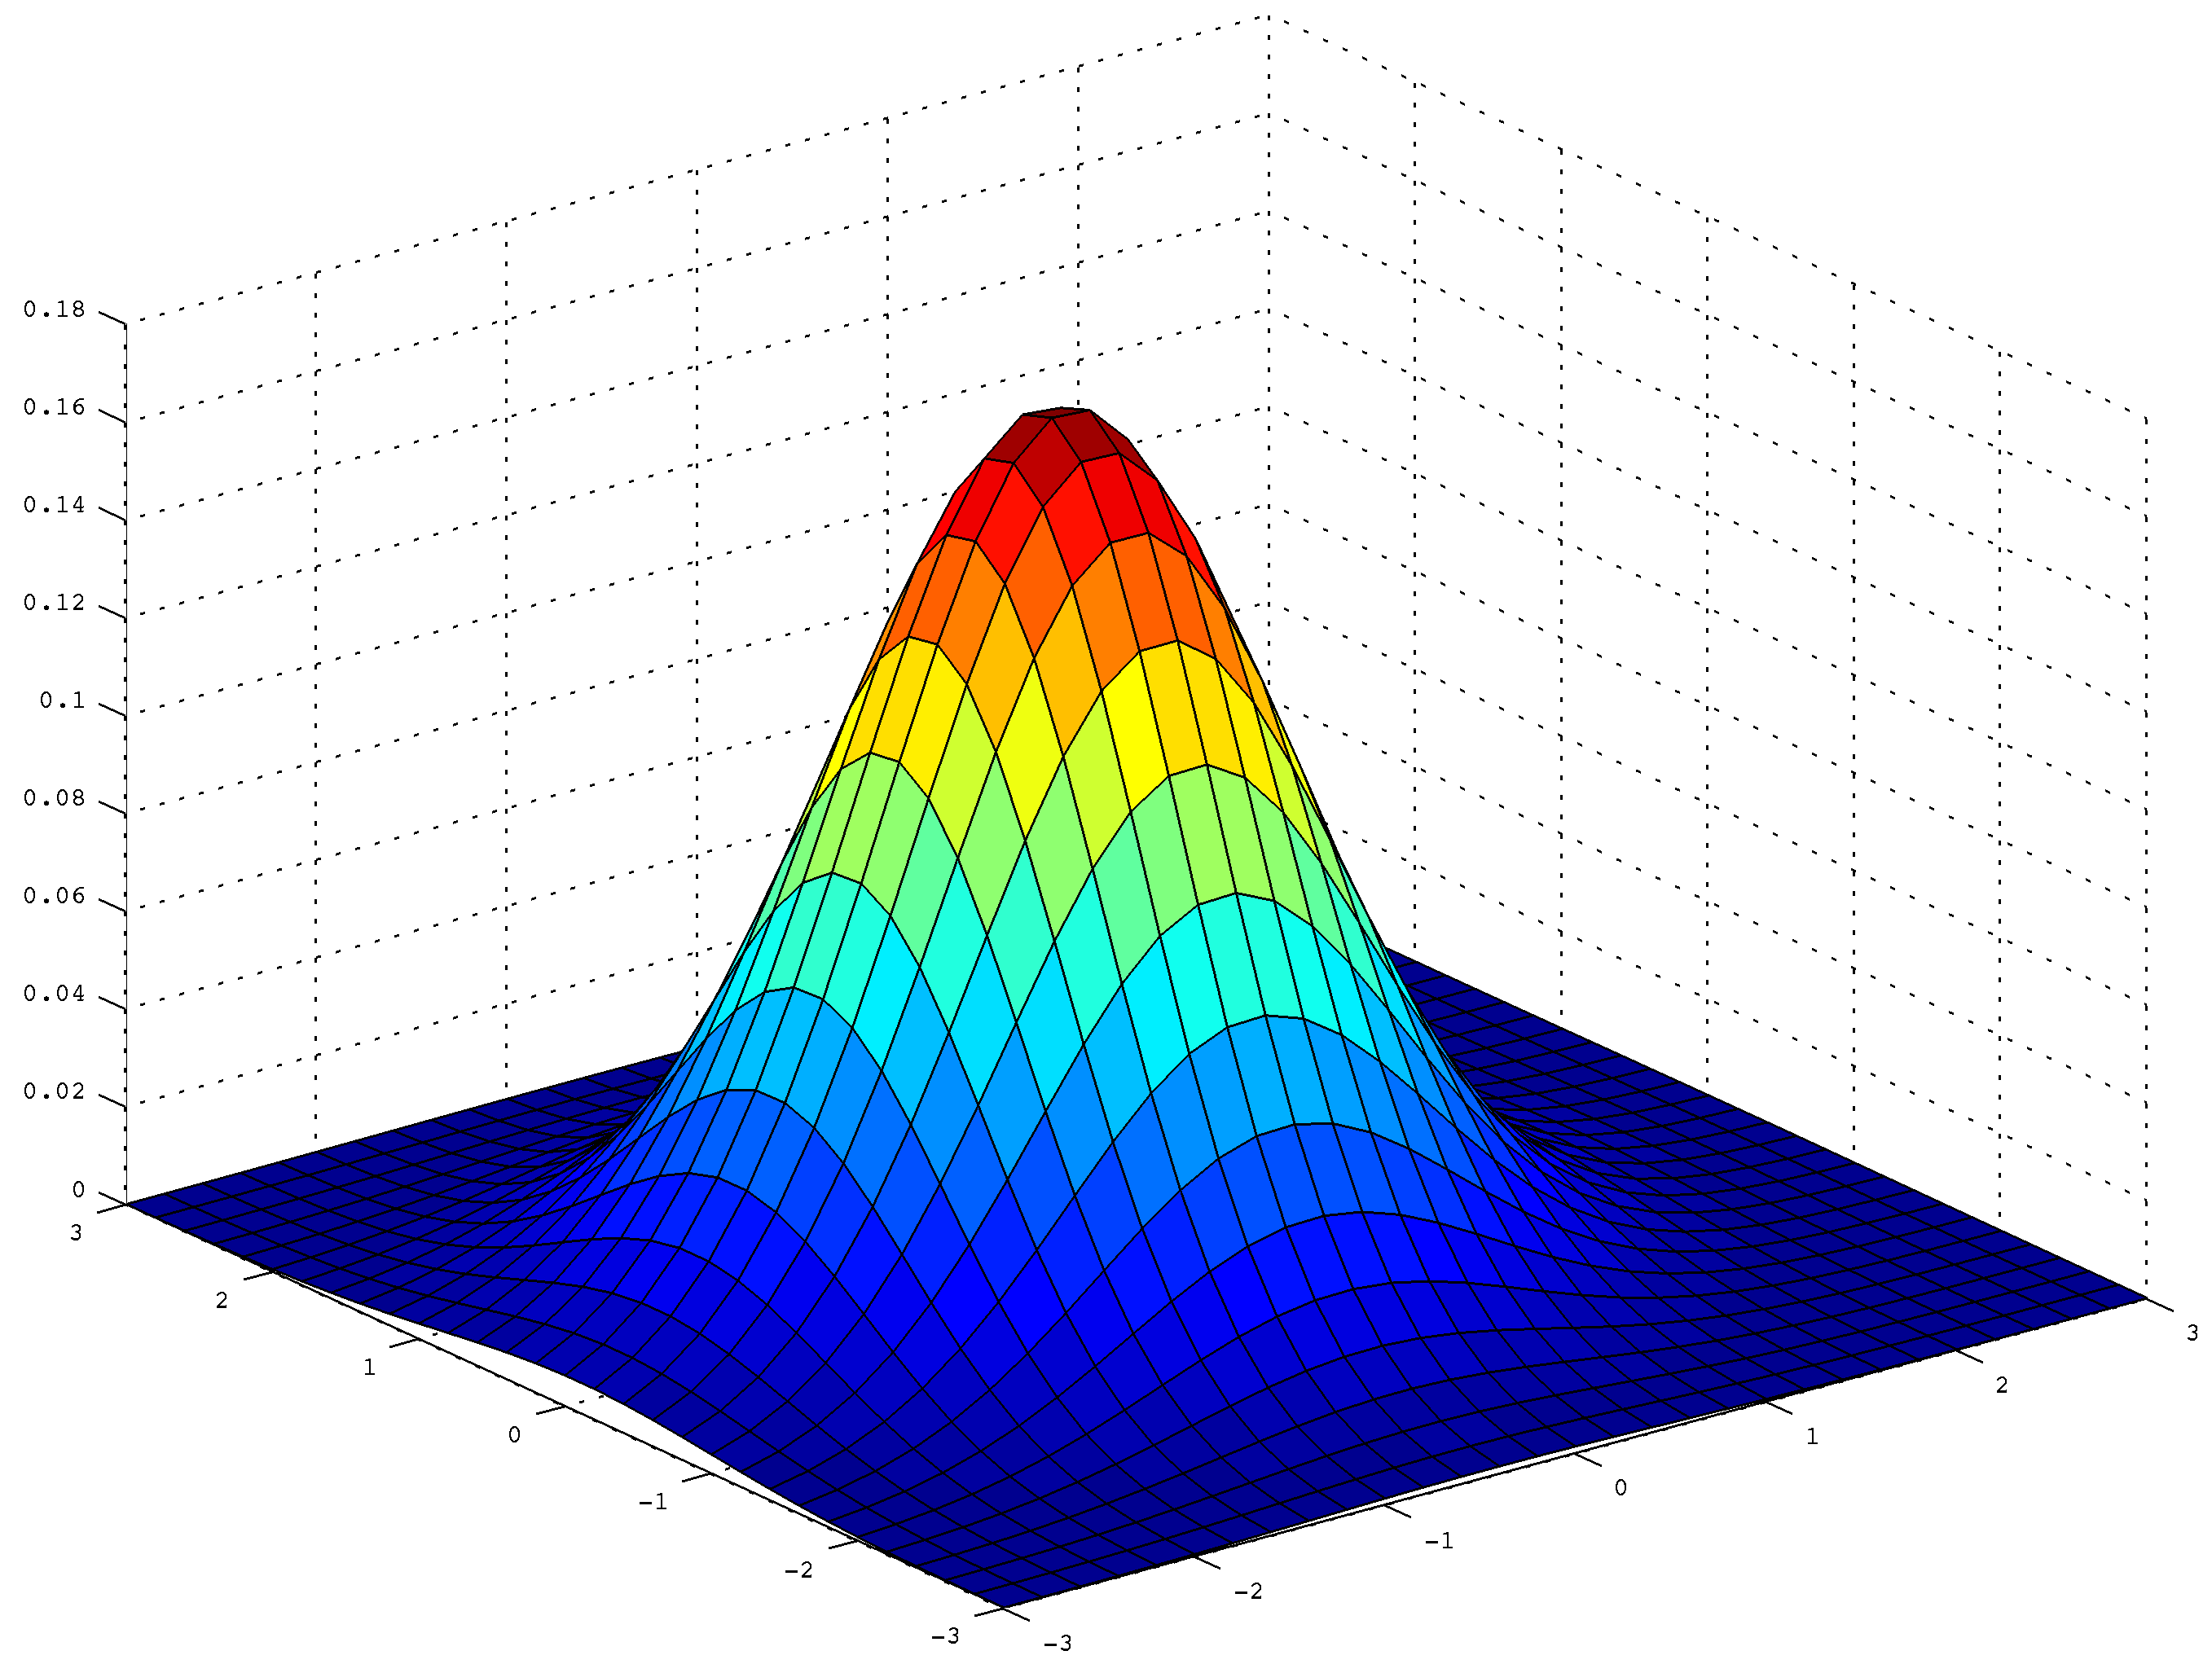
\includegraphics[width=0.7\textwidth]{gaussian-pdf.png}
	\caption{Bivariate Gaussian distribution (\href{https://stats.stackexchange.com/questions/102632/plot-two-dimensional-gaussian-density-function-in-matlab}{src}).}
	\label{fig:relation-ai-ml-dl}
\end{figure}

\subsection{Multivariate Normal Distribution}
\textit{Multivariate Normal Distribution} is the extension of \textit{Univariate Normal Distribution} to multi-dimensional data: $\textbf{x}, \boldsymbol{\mu} \in \mathbb{R}^D, \sigma^2 \Rightarrow \Sigma \in \mathbb{S}^D_{++}$ ($\mathbb{S}^D_{++}$ is the set of positive definite symmetric matrix)
\begin{equation}
	p(x) = \text{Norm}_x [\boldsymbol{\mu}, \Sigma] = \mathcal{N}(\boldsymbol{\mu}, \Sigma) = \frac{1}{2\pi^{D/2}| \Sigma|^{\frac{1}{2}}} . \text{exp} \left( -\frac{1}{2} {(\textbf{x} - \boldsymbol{\mu})^T \Sigma^{-1} (\textbf{x} - \boldsymbol{\mu})} \right)
\end{equation}

\subsection{Beta Distribution}
This distribution describes the parameter for another distributions. \Eg, Dirichlet \ac{pdf} describes Categorical Distribution (\subsecref{subsec:categorical-distribution})

\section{Parameter Estimation}
Many of \ac{ML} problems are boiled down to finding \textit{statistical models}. Those models could predict the \ac{prob} for the classification problem, \ac{prob} of events that will happen, \etc. It all end up with finding the suitable set of \ac{param} for these \textit{statistical models}.
\subsection{Maximum Likelihood Estimation}
\ac{MLE} finds the parameters that maximize the \ac{prob} of the existing data.
\begin{align}
	& &&\theta = \underset{\theta}{\text{argmax}}\:p(x_1, x_2, \dots, x_N | \theta) \\
	&\text{Assuming independent variables:} &&\theta = \underset{\theta}{\text{argmax}} \prod^N_{n=1} p(x_n | \theta) \\
	&\text{Maximum log-likelihood:} &&\theta = \underset{\theta}{\text{argmax}} \sum^N_{n=1} \left[\text{log}\:p(x_n | \theta) \right]\\
	&\text{Minimum negative log-likelihood:} && \theta = \underset{\theta}{\text{argmin}} \sum^N_{n=1} \left[-\text{log}\:p(x_n | \theta)\right]
\end{align}

\subsection{Maximum A Posteriori}
Sometimes, we have prior knowledge of the \ac{pdf}. \Eg, we know that the \ac{prob} of getting head when flipping a coin is around 50\%. \ac{MAP} takes advantage of the prior knowledge $p(\theta)$ on the parameters $\theta$ by applying Bayes rule (\subsecref{subsec:bayes-rule})
\begin{equation}
	\theta = \underset{\theta}{\text{argmax}} \prod^N_{n=1} p(x_n | \theta)p(\theta)
\end{equation}
\hlr{\ac{MLE} suffers when there is not enough data} $\Rightarrow$ \hlr{use \ac{MAP}}

\section{Naive Bayes Classifier}
Naive implies having the independence assumption on the variables.
\begin{align*}
	c 	&= \underset{c \in \mathbb{C}}{\text{argmax}}\:p(c|x)\\
		&= \underset{c \in \mathbb{C}}{\text{argmax}}\:p(x|c)\,p(c)
\end{align*}

If $x$ is:
\begin{itemize}
	\item continuous variable $\Rightarrow$ Gaussian Naive Bayes
	\item feature vector $\Rightarrow$ Multinomial Naive Bayes
	\item binary vector $\Rightarrow$ Bernoulli Naive Bayes
\end{itemize}

Minimize the expected loss: $\displaystyle \expectation{L} = \sum_{k}\sum_{j}\int_{R_j}L_{kj}\,p(x, C_k)\,dx$ by choosing region $R_j$ such that $\displaystyle \expectation{L} = \sum_kL_{kj}\,p(C_k| x)$

\section{Views on the Decision Problem}
\subsection{\hlr{Generative Methods}}
First determine the class-conditional densities and separately infer the prior class \ac{prob} $\Rightarrow$ Bayes theorem $\Rightarrow$ class membership
\[p(x|C_k)\,p(C_k) \Rightarrow y_k(x)\]
\Eg, Mixture of Gaussians

\subsection{\hlr{Discriminative Methods}}
First solve the inference problem of determined the posterior class \ac{prob}

\section{Unknown Notes}
\Eg, 2 class $C_1, \; C_2$, 2 decisions $\alpha_1, \; \alpha_2$.

The loss: $L(\alpha_j | C_k) = L_{kj}$.

The expected loss is equal to the $Risk(R)$.
\begin{align*}
	\mathbb{E}_{\alpha_1}[L] = R(\alpha_1|x) = L_{11}\,p(C_1|x) + L_{21}\,p(C_2|x)\\
	\mathbb{E}_{\alpha_2}[L] = R(\alpha_2|x) = L_{12}\,p(C_1|x) + L_{22}\,p(C_2|x)\\
\end{align*}
Choose $\alpha_1$ if $R(\alpha_1|x) < R(\alpha_2|x)$

% !TeX spellcheck = en_US

\section{Probability Density Estimation}
\label{cha:pdf-estimation}

\subsection{Histogram}
This is \hlb{non-parametric} \ac{prob} density estimation. All other approaches are \hlb{parametric}. The \ac{prob} of a bin:
\begin{equation}
	p_i = \frac{n_i}{N.\Delta_i}
\end{equation}

in which $n_i$ is the number of data points in that bin, $N$ is the total number of data point, $\Delta_i$ is the width of the bin, often $\Delta_i=\Delta$.

\hlb{Notes}:
\begin{itemize}
	\item $\Delta$ serves as the \hlr{smoothing factor}
	\item With $D$ as the dimensions of the data points. The number of bins grow exponentially with $\mathcal{O}(k^D)$
\end{itemize}
\begin{figure}[hbt!]
	\centering
	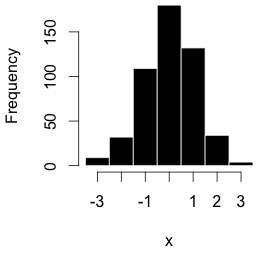
\includegraphics[width=0.4\textwidth]{histogram.png}
	\caption{Example of a histogram, $\Delta = 1$ (\href{https://en.wikipedia.org/wiki/Histogram}{src}).}
\end{figure}

\subsection{Parametric Probability Density Estimation}
In the other hands, one could find the \ac{prob} from $\displaystyle p = \int_{\mathcal{R}}p(y)dy \approx p(x)V$ where the region $\mathcal{R}$ is sufficiently small.\\
$\displaystyle \Rightarrow p(x) \approx \frac{K}{N.V}$, where $K$ is the number of data points in the region, $V$ is the volume of the region.

\subsection{Kernel Methods}
The kernel methods fix $V$ and determine $K$. The volume $V$ is the space restricted within a parzen window $k(u)$ that satisfies $k(u) \geq 0$.
\begin{align}
	&\text{A hyper-space cube:} && k(u) = \begin{cases}
		1\;\; if \;\; |u_i| \leq \frac{1}{2}h, \;\; i = 1, 2, \dots, D \\
		0\;\; else
	\end{cases} \\
	&\text{The number of points inside:} &&K = \sum_{n=1}^{N} k(x-x_n) \\
	&\text{The region \textit{volume}:} &&V = \int k(u) du = h^D\\
	&\text{The probability:} && \Rightarrow p(x) \approx \frac{K}{N.V} = \frac{1}{N.h^D}\sum_{n=1}^{N}k(x-x_n)
\end{align}
The \hlb{symmetric Gaussian kernel is a better substitution} for the asymmetric parzen window.
\begin{align}
	&\text{A Gaussian kernel:} && k(u) = \frac{1}{\sqrt{2\pi h^2}}\:exp\left(\frac{-u^2}{2h^2}\right) \\
	&\text{The region \textit{volume}:} &&V = \int k(u) du = 1 \\
	&\text{The probability:} && \Rightarrow p(x) \approx \frac{1}{N} \sum_{n=1}^{N} \frac{1}{(2\pi)^{D/2}h}\:exp\left(\frac{-||x-x_n||^2}{2h^2}\right)
\end{align}
For Kernel methods, $h$ is the \hlb{smoothing factor}.

Generalization: $k(u) \geq 0$, $\displaystyle \int k(u)du = 1$.

\hlr{Size of the hypersphere is proportional to $h^2$.}

\subsection{K-Nearest Neighbor}
When you fix $K$ and determine $V$, it leads to K-Nearest Neighbor.

\todo{Add image}

\begin{equation}
	p(x) \approx \frac{K}{NV}
\end{equation}
Here, $K$ is the \hlb{smoothing factor}.

\hlr{\begin{itemize}
		\item Too much bias $\Rightarrow$ too smooth
		\item Too much variance $\Rightarrow$ \underline{NOT} smooth enough
	\end{itemize}
	$\Rightarrow$ combine parametric methods to a mixture model}

\hlr{Mixture distribution = multi parametric model}

\subsection{Mixture of Gaussians}
\ac{MoG}, as \hlr{Generative Model}, is defined from the \ac{prob} sum of elemental Gaussians: $\displaystyle p(x|\theta) = \sum_{j=1}^{M}p(x|\theta_j)p(j)$, where $p(x|\theta_j)$ is a \hlr{mixture component}, $p(j) = \pi_j$ is the \hlr{weight of the component}
\begin{align}
	p(x|\theta_j) &= \frac{1}{\sqrt{2\pi}\sigma_j}\:exp\left[\frac{-(x-\mu_j)^2}{2\sigma_j^2}\right],\;\;p(j)=\pi_j, \;\;\sum\pi_j=1 \\
	p(x|\theta_j) &= \frac{1}{(2\pi)^{\frac{D}{2}}|\Sigma_j|^{\frac{1}{2}}}\:exp\left[-\frac{1}{2}(x-\mu_j)^T\Sigma_j^{-1}(x-\mu_j)\right]
\end{align}

\subsection{K-Means Clustering}
There are 3 steps:
\begin{itemize}
	\item Pick $K$ centroids
	\item Assign sample to the centroid
	\item Adjust centroids
\end{itemize}

Step 2 and 3 are repeated until there is no change.

This leads to a local optimum, depends on initialization. It's sensitive to \hlb{outliers}, detects \hlb{spherical clusters only}.

\todo{Add images}

Application: \eg, image compression.

\subsection{EM Clustering}
It's short for Expectation-Maximization. Assuming $N$ data points and $K$ Gaussians.
\begin{itemize}
	\item \textbf{E-Step:} Fix the Gaussians, find $\gamma_j(x)$, which represent the \hlr{responsibility of component $j$ for $x$}.
	\begin{equation}
		\gamma_j(x_n) = \frac{\pi_j \mathcal{N}\left(x_n|\mu_j,\Sigma_j\right)}
		{\sum_{k=1}^{K}\pi_k \mathcal{N}\left(x_n|\mu_k,\Sigma_k\right)} \;\;\forall j=1, 2, \dots, K, \;\; n=1, 2, \dots, N
	\end{equation}	
	\item \textbf{M-Step:} Fix $\gamma_j(x)$, update the Gaussians.
	\begin{align}
		\hat{N}_j &= \sum_{n=1}^{N}\gamma_j(x_n) \\
		\hat{\mu}_j &= \frac{1}{\hat{N}_j} \sum_{n=1}^{N} \gamma_j(x_n)x_n \\
		\hat{\pi}_j &= \frac{\hat{N}_j}{N} \\
		\hat{\Sigma}_j &= \frac{1}{\hat{N}_j} \sum_{n=1}^{N} \gamma_j(x_n) \left(x_n - \hat{\mu}_j\right)\left(x_n - \hat{\mu}_j\right)^T
	\end{align}
\end{itemize}
\hlb{Notes}:
\begin{itemize}
	\item Regularization with $\Sigma + \sigma_{min}I$
	\item Initialization $\mu_j$ with K-Means
	\item Hard-assignment: each data point to 1 class $\Rightarrow$ K-Means
	\item Soft-assignment: each data point $\Rightarrow$ \ac{prob} to fall into many classes $\Rightarrow$ EM Clustering
\end{itemize}

EM \hlr{needs more iteration}, because there are \hlr{more \ac{param}}.